% Licensed to the Apache Software Foundation (ASF) under one
% or more contributor license agreements.  See the NOTICE file
% distributed with this work for additional information
% regarding copyright ownership.  The ASF licenses this file
% to you under the Apache License, Version 2.0 (the
% "License"); you may not use this file except in compliance
% with the License.  You may obtain a copy of the License at

%   http://www.apache.org/licenses/LICENSE-2.0

% Unless required by applicable law or agreed to in writing,
% software distributed under the License is distributed on an
% "AS IS" BASIS, WITHOUT WARRANTIES OR CONDITIONS OF ANY
% KIND, either express or implied.  See the License for the
% specific language governing permissions and limitations
% under the License.

!TEX root = ../design.tex


\chapter[k Nearest Neighbors]{k Nearest Neighbors}

\begin{moduleinfo}
\item[Authors] \href{mailto:okislal@pivotal.io}{Orhan Kislal}

\item[History]
	\begin{modulehistory}
		\item[v0.1] Initial version: knn and kd-tree.
	\end{modulehistory}
\end{moduleinfo}


% Abstract. What is the problem we want to solve?
\section{Introduction} % (fold)
\label{sec:knn_introduction}

\emph{Some notes and figures in this section are borrowed from \cite{medium_knn} and \cite{point_knn}}.

K-nearest neighbors (KNN) is one of the most commonly used learning
algorithms. The goal of knn is to find a number (k) of training data points
closest to the test point. These neighbors can be used to predict labels via
classification or regression.

KNN does not have a training phase like the most of learning techniques. It
does not create a model to generalize the data, instead the algorithm uses the
whole training dataset (or a specific subset of it).

KNN can be used for classification, the output is a class membership (a
discrete value). An object is classified by a majority vote of its neighbors,
with the object being assigned to the class most common among its k nearest
neighbors. It can also be used for regression, output is the value for the
object (predicts continuous values). This value is the average (or median) of
the values of its k nearest neighbors.

\section{Implementation Details}

The basic KNN implementation depends on the table join between the training dataset and the test dataset.

\begin{sql}
	(SELECT test_id,
            train_id,
            fn_dist(train_col_name, test_col_name) AS dist,
            label
    FROM train_table, test_table) AS knn_sub
\end{sql}

Once we have the distance between every train - test pair, the algorithm picks the k smallest values.

\begin{sql}
	SELECT row_number() OVER
        (PARTITION BY test_id ORDER BY dist) AS r,
        test_id,
        train_id,
        label
	FROM knn_sub
	WHERE r <= k
\end{sql}

Finally, the prediction is completed based on the labels of the selected
training points for each test point.

\section{Enabling KD-tree}

One of the major shortcomings of KNN is the fact that it is computationally
expensive. In addition, there is no training phase; which means every single
prediction will have to compute the full table join. One of the ways to
improve the performance is to reduce the search space for test points. Kd-tree
option is developed to enable trading the accuracy of the output with higher
performance by reducing the neighbor search space.

Kd-trees are used for organizing data in k dimensions. It is constructed like
a binary search tree where each level of the tree is using a specific
dimension for finding splits.


\begin{figure}[h]
	\centering
	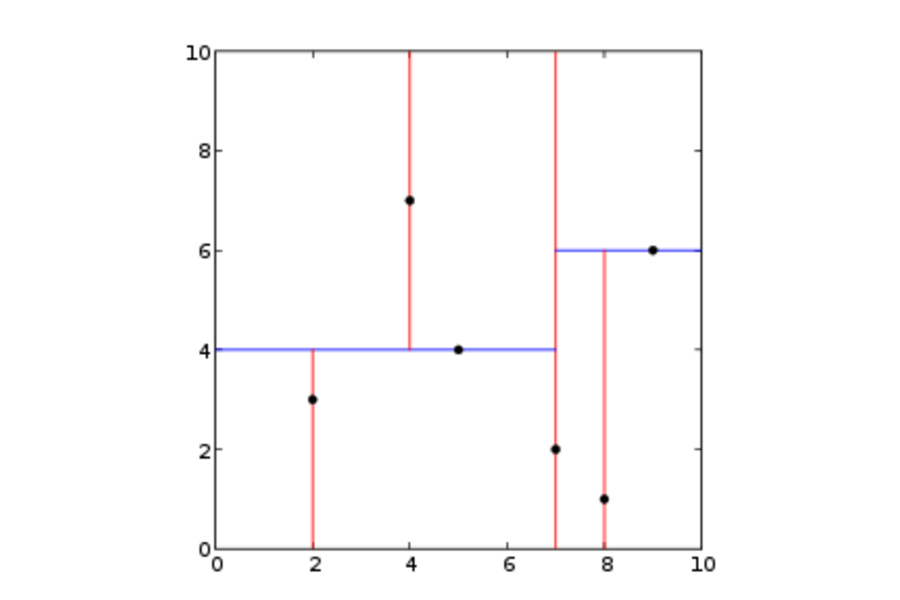
\includegraphics[width=0.9\textwidth]{figures/2d_kdtree.pdf}
\caption{A 2D kd-tree of depth 3}
\label{kdd:2d_kdtree}
\end{figure}

A kd-tree is constructed by finding the median value of the data in a
particular dimension and separating the data into two sections based on this
value. This process is repeated a number of times to construct smaller
regions. Once the kd-tree is prepared, it can be used by any test point to
find its assigned region and this fragmentation can be used for limiting the
search space for nearest neighbors.

Once we have the kd-tree regions and their borders, we find the associated
regions for the test points. This gives us the first region to search for
nearest neighbors. In addition, we allow the user to request for multiple
regions to search. This means we have to decide which additional regions to
include in our search. We implemented a backtracking algorithm to find these
regions. The core idea is to find the closest border for each test point and
select the region on the other side of the border. Note that points that
reside in the same region might have different secondary (or tertiary, etc.)
regions. Consider the tree at Figure~\ref{kdd:2d_kdtree}. A test point at $<5
, 2>$ is in the same region as $<3 , 3.9>$. However, their closest borders and
the associated secondary regions are wildly different. In addition, consider
$<3 , 3.9>$ and $<6 , 3.9>$. They both have the same border as their closest
one ($y=4$). However, their closest regions do differ. To make sure that we
get the correct region, the following scheme is implemented. For a given point
$P$, we find the closest border, $dim[i] = x$ and $P$'s relative position to
it ($pos$ = $-1$ for lower and $+1$ for higher). We conjure a new point that
consists of the same values as the test point in every dimension except $i$.
For $dim[i]$, we set the value to $x-pos*\epsilon$. Finally, we use the
existing kd-tree to find this new point's assigned region. This region is our
expansion target for the point $P$. We repeat this process with the next
closest border as requested by the user.

The knn algorithm does not change significantly with the addition of regions.
Assuming that the training and test datasets have their region information
stored in the tables, the only necessary change is ensuring that the table
join uses these region ids to limit the search space.


\begin{sql}
	(SELECT test_id,
            train_id,
            fn_dist(train_col_name, test_col_name) AS dist,
            label
    FROM train_table, test_table
    WHERE train_table.region_id = test_table.region_id
    ) AS knn_sub
\end{sql}
